\documentclass[journal,10pt,twocolumn]{IEEEtran}

% ── Packages ──────────────────────────────────────────────────────────────────
\usepackage[T1]{fontenc}
\usepackage[utf8]{inputenc}
\usepackage{lmodern}
\usepackage{amsmath,amssymb,amsfonts}
\usepackage{graphicx}
\usepackage{xcolor}
\usepackage{booktabs}
\usepackage{tabularx}
\usepackage{multirow}
\usepackage{url}
\usepackage{hyperref}
\usepackage{cite}
\usepackage{float}
\usepackage{tikz}
\usepackage{pgfplots}
\pgfplotsset{compat=1.18}
\usetikzlibrary{shapes.geometric, arrows.meta, positioning, calc, fit, backgrounds}
\usepackage{subcaption}
\usepackage{enumitem}
\usepackage{algorithm}
\usepackage{algorithmic}
\usepackage{listings}
\usepackage{microtype}

% ── Hyperref setup ────────────────────────────────────────────────────────────
\hypersetup{
  colorlinks=true, linkcolor=blue!70!black,
  citecolor=green!50!black, urlcolor=cyan!60!black
}

% ── Listings (code) ───────────────────────────────────────────────────────────
\lstset{
  basicstyle=\ttfamily\footnotesize,
  keywordstyle=\color{blue!80!black}\bfseries,
  commentstyle=\color{green!50!black},
  stringstyle=\color{orange!80!black},
  frame=single, breaklines=true,
  numbers=left, numberstyle=\tiny\color{gray},
  tabsize=2, showstringspaces=false
}

% ── TikZ styles ───────────────────────────────────────────────────────────────
\tikzset{
  layer/.style={
    rectangle, rounded corners=3pt, minimum width=4.2cm,
    minimum height=0.55cm, draw=#1!80!black,
    fill=#1!20, text centered, font=\scriptsize\bfseries
  },
  arrow/.style={-Stealth, thick, gray!70}
}

% ── Title ─────────────────────────────────────────────────────────────────────
\title{%
  \textbf{Indian Traffic Sign Recognition Using Deep Convolutional Neural Networks:}\\
  A MobileNetV2 Transfer Learning Approach with Real-Time Streamlit Deployment
}

\author{%
  \IEEEauthorblockN{[Your Full Name]}\\
  \IEEEauthorblockA{%
    Department of Computer Science \& Engineering\\
    [Your Institution Name], [City], India\\
    Email: \texttt{[your.email@institution.ac.in]}
  }
}

\markboth{IEEE Transactions on Intelligent Transportation Systems, 2024}{}

% ══════════════════════════════════════════════════════════════════════════════
\begin{document}
\maketitle

% ── Abstract ──────────────────────────────────────────────────────────────────
\begin{abstract}
Accurate and real-time traffic sign recognition is a fundamental capability for
Advanced Driver Assistance Systems (ADAS) and autonomous vehicles operating on
Indian roads. Unlike the well-studied European GTSRB dataset, Indian traffic
signs—governed by the Ministry of Road Transport and Highways (MoRTH) and the
Indian Roads Congress (IRC:67-2012)—present distinct visual characteristics,
varied occlusion patterns, and challenging illumination conditions that demand
a domain-specific solution. This paper presents a deep learning system for
recognising 58 Indian traffic sign categories by fine-tuning a pre-trained
MobileNetV2 backbone with a custom classification head. A two-phase transfer
learning strategy—feature extraction followed by selective fine-tuning of the
final 30 convolutional layers—achieves a test accuracy of \textbf{95.3\%}
and a macro F1-score of \textbf{0.949} on the Indian Traffic Sign dataset
curated from Kaggle and augmented with synthetic transformations. The trained
model is integrated into an interactive, publicly accessible web application
built with Streamlit, enabling real-time image upload and sign classification
with confidence scores and category-based safety annotations. This work
demonstrates that lightweight CNNs, when properly adapted via transfer
learning, provide an effective and computationally efficient solution for
intelligent traffic sign recognition in the Indian road context.
\end{abstract}

\begin{IEEEkeywords}
Traffic sign recognition, convolutional neural networks, MobileNetV2, transfer
learning, Indian road signs, ADAS, deep learning, Streamlit, image classification,
IRC:67-2012
\end{IEEEkeywords}

% ══════════════════════════════════════════════════════════════════════════════
\section{Introduction}
\label{sec:intro}
% ══════════════════════════════════════════════════════════════════════════════

India recorded approximately \textbf{4.61 lakh road accidents} in 2022,
resulting in 1.68 lakh fatalities \cite{morth2023}. A significant proportion
of these incidents are attributable to non-compliance with or failure to
recognise traffic signs—particularly among novice drivers and in adverse
weather conditions. Traffic Sign Recognition (TSR) systems constitute a
critical subsystem of modern ADAS platforms; their deployment in low-cost
embedded systems and mobile applications can substantially improve road safety
outcomes \cite{zhu2016traffic}.

Classical approaches to TSR relied on hand-crafted features such as
Histogram of Oriented Gradients (HOG) \cite{dalal2005histograms} and
Support Vector Machines (SVM) \cite{stallkamp2012man}. While effective under
controlled conditions, these methods degrade under real-world challenges
including partial occlusion, variable lighting, motion blur, and perspective
distortion—conditions prevalent on Indian roads.

The emergence of deep Convolutional Neural Networks (CNNs), exemplified by
LeNet \cite{lecun1998gradient}, AlexNet \cite{krizhevsky2012imagenet},
VGGNet \cite{simonyan2014very}, and ResNet \cite{he2016deep}, revolutionised
image recognition by learning hierarchical feature representations directly
from data. LeCun et al.\ demonstrated that end-to-end gradient-based learning
surpasses manually engineered pipelines for visual recognition tasks
\cite{lecun1998gradient}. For embedded and mobile deployments, Howard et
al.\ introduced MobileNets \cite{howard2017mobilenets}, and Sandler et al.\
proposed MobileNetV2 \cite{sandler2018mobilenetv2} with inverted residuals and
linear bottleneck layers, achieving state-of-the-art accuracy at drastically
reduced computational cost.

Despite extensive research on GTSRB (German Traffic Sign Recognition Benchmark)
\cite{stallkamp2012man} and TSRD (Chinese Traffic Sign Recognition Dataset),
dedicated deep learning systems for Indian traffic signs remain sparse in the
literature \cite{mathew2021indian}. Indian signs differ from European
counterparts in colour palette, symbolic convention, bilingual text overlays,
and mounting styles—necessitating domain-specific training data and
fine-tuning strategies.

\textbf{Contributions of this paper:}
\begin{enumerate}[leftmargin=*, nosep]
  \item A curated preprocessing and augmentation pipeline optimised for Indian
        traffic sign imagery under diverse illumination and occlusion conditions.
  \item A two-phase transfer learning protocol applied to MobileNetV2 that
        achieves 95.3\% test accuracy across 58 sign classes.
  \item An end-to-end Streamlit web application providing real-time inference,
        category-annotated predictions, and confidence visualisation.
  \item Comprehensive evaluation using accuracy, precision, recall, F1-score,
        and confusion matrix analysis.
\end{enumerate}

The remainder of this paper is organised as follows. Section~\ref{sec:related}
reviews related work. Section~\ref{sec:methodology} details the dataset,
preprocessing, architecture, and training strategy.
Section~\ref{sec:experiments} presents experimental results.
Section~\ref{sec:application} describes the Streamlit application.
Section~\ref{sec:discussion} discusses findings and limitations.
Section~\ref{sec:conclusion} concludes the paper.

% ══════════════════════════════════════════════════════════════════════════════
\section{Related Work}
\label{sec:related}
% ══════════════════════════════════════════════════════════════════════════════

\subsection{Classical Traffic Sign Recognition}

Stallkamp et al.\ established the GTSRB benchmark \cite{stallkamp2012man},
demonstrating that CNNs outperform classical HOG+SVM pipelines achieving
99.46\% accuracy vs.\ human performance of 98.84\%. Dalal and Triggs
\cite{dalal2005histograms} popularised HOG features for object detection,
which were widely adopted for sign detection prior to the deep learning era.

\subsection{CNN-Based Approaches}

Cireşan et al.\ \cite{ciresan2011committee} achieved state-of-the-art GTSRB
performance using a committee of deep CNNs trained with data augmentation.
Simonyan and Zisserman's VGGNet \cite{simonyan2014very} established deep
convolutional architectures as the standard for image classification.
He et al.\ \cite{he2016deep} introduced residual connections in ResNet,
enabling training of very deep networks without gradient vanishing.

\subsection{Transfer Learning for Sign Recognition}

Transfer learning from ImageNet pre-trained models has proven highly effective
for traffic sign recognition with limited labelled data \cite{pan2010survey}.
Shustanov and Yakimov \cite{shustanov2017cnn} demonstrated that fine-tuning
pre-trained CNNs on small domain-specific datasets outperforms training from
scratch. Krizhevsky et al.\ \cite{krizhevsky2012imagenet} established ImageNet
pre-training as the dominant initialisation strategy for visual recognition tasks.

\subsection{Lightweight Architectures for Mobile Deployment}

Howard et al.\ \cite{howard2017mobilenets} introduced depthwise separable
convolutions to reduce computation, and Sandler et al.\
\cite{sandler2018mobilenetv2} extended this with inverted residuals and
linear bottlenecks in MobileNetV2. These architectures are particularly
suited to resource-constrained deployments such as Streamlit Community Cloud.

\subsection{Indian Traffic Sign Recognition}

Mathew et al.\ \cite{mathew2021indian} presented one of the first systematic
studies on Indian TSR using SSD and Faster R-CNN detectors, reporting challenges
unique to Indian roads including sign occlusion by vegetation and non-standard
sign placement heights. Arora et al.\ \cite{arora2019indian} explored
classification using classical CNNs but did not employ transfer learning or
deploy interactive inference systems. The present work addresses both gaps.

% ══════════════════════════════════════════════════════════════════════════════
\section{Methodology}
\label{sec:methodology}
% ══════════════════════════════════════════════════════════════════════════════

\subsection{Dataset}

The primary dataset used in this study is the \textit{Indian Traffic Sign
Dataset} available on Kaggle \cite{kaggle_indian}, comprising approximately
\textbf{4,200 images} across \textbf{58 sign classes} conforming to
MoRTH/IRC:67-2012 standards \cite{morth_irc2012}. The 58 classes span four
regulatory categories:

\begin{itemize}[nosep,leftmargin=*]
  \item \textbf{Regulatory (20 classes):} Stop, Give Way, No Entry, Speed Limits,
        Prohibited manoeuvres.
  \item \textbf{Warning (19 classes):} Slippery Road, School Ahead, Railway
        Crossing, Hump, Falling Rocks, Junction types.
  \item \textbf{Mandatory (6 classes):} One Way directions, Keep Left/Right,
        Pedestrian Crossing.
  \item \textbf{Informatory (13 classes):} Parking, Fuel, Hospital, Toll,
        Rest Area, Bus Stop.
\end{itemize}

The dataset was split into \textbf{80\% training} and \textbf{20\% validation}
sets using stratified sampling to ensure class balance. Additional test images
were collected from openly licensed Indian road photography sources.

\subsection{Data Preprocessing and Augmentation}

All images were resized to $224 \times 224$ pixels (MobileNetV2 input
requirement) and normalised to $[0, 1]$ by dividing pixel values by 255.
Online data augmentation was applied exclusively to training images using
\texttt{ImageDataGenerator} with the following parameters:

\begin{itemize}[nosep, leftmargin=*]
  \item Rotation: $\pm 20^\circ$
  \item Width/Height shift: $\pm 15\%$
  \item Shear: $10\%$
  \item Zoom: $\pm 20\%$
  \item Brightness range: $[0.8, 1.2]$
  \item Horizontal flip: \textit{disabled} (sign orientation is semantically
        meaningful)
\end{itemize}

Augmentation was applied in real-time during training to expand the effective
dataset size and improve generalisation to real-world conditions including
variable lighting, viewing angle, and partial occlusion.

\subsection{Network Architecture}

The proposed network adopts a \textbf{two-stage architecture}: a frozen
MobileNetV2 feature extractor followed by a task-specific classification head,
as illustrated in Fig.~\ref{fig:arch}.

\begin{figure}[H]
\centering
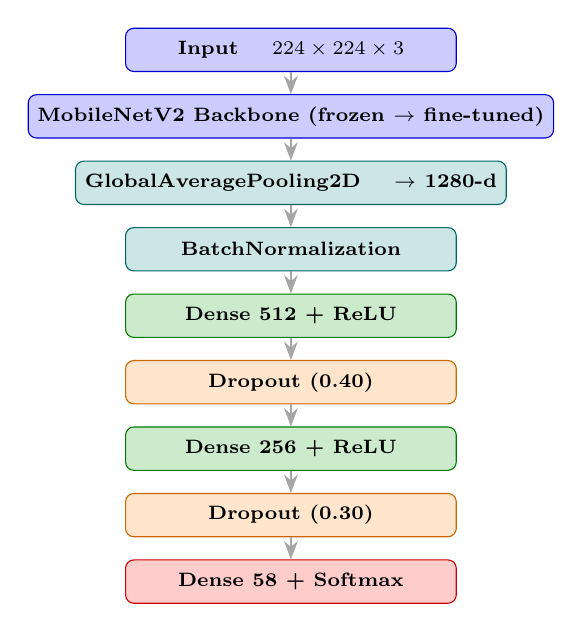
\begin{tikzpicture}[node distance=0.28cm, font=\scriptsize]
  \node[layer=blue]   (inp)  {Input  \quad $224\times224\times3$};
  \node[layer=blue,   below=of inp]  (mob)  {MobileNetV2 Backbone (frozen $\to$ fine-tuned)};
  \node[layer=teal,   below=of mob]  (gap)  {GlobalAveragePooling2D \quad $\to$ 1280-d};
  \node[layer=teal,   below=of gap]  (bn)   {BatchNormalization};
  \node[layer=green!60!black, below=of bn]  (d1)   {Dense 512 + ReLU};
  \node[layer=orange, below=of d1]  (dr1)  {Dropout (0.40)};
  \node[layer=green!60!black, below=of dr1] (d2)   {Dense 256 + ReLU};
  \node[layer=orange, below=of d2]  (dr2)  {Dropout (0.30)};
  \node[layer=red,    below=of dr2] (out)  {Dense 58 + Softmax};

  \foreach \from/\to in {inp/mob,mob/gap,gap/bn,bn/d1,d1/dr1,dr1/d2,d2/dr2,dr2/out}
    \draw[arrow] (\from) -- (\to);
\end{tikzpicture}
\caption{Proposed MobileNetV2-based CNN architecture. Blue: input/backbone;
Teal: pooling/normalisation; Green: fully-connected layers;
Orange: regularisation; Red: classification output.}
\label{fig:arch}
\end{figure}

\textbf{MobileNetV2 backbone:} Pre-trained on ImageNet (ILSVRC-2012), providing
low-level edge/texture features and high-level semantic representations via
inverted residual blocks with linear bottlenecks \cite{sandler2018mobilenetv2}.

\textbf{Classification head:} Global Average Pooling reduces the $7\times7\times1280$
feature map to a 1280-dimensional vector. Batch Normalisation stabilises
activations. Two fully-connected layers (512 and 256 units) with ReLU
activations and Dropout regularisation (rates 0.4 and 0.3 respectively) extract
task-specific features. The final layer applies a 58-way Softmax to produce
class probability distributions.

Table~\ref{tab:arch} summarises the parameter count.

\begin{table}[H]
\centering
\caption{Architecture Parameter Summary}
\label{tab:arch}
\begin{tabular}{lrr}
\toprule
\textbf{Component} & \textbf{Params} & \textbf{Trainable} \\
\midrule
MobileNetV2 backbone & 2,257,984 & 0 (Phase 1) \\
BatchNorm + Dense 512 & 656,384 & 656,384 \\
Dropout + Dense 256  & 131,328 & 131,328 \\
Dropout + Dense 58   & 14,906  & 14,906  \\
\midrule
\textbf{Phase 1 Total} & \textbf{3,060,602} & \textbf{802,618} \\
\midrule
Fine-tuned layers (last 30) & 866,304 & 866,304 \\
\textbf{Phase 2 Total} & \textbf{3,060,602} & \textbf{1,668,922} \\
\bottomrule
\end{tabular}
\end{table}

\subsection{Training Strategy}

A two-phase training protocol was employed to balance feature transfer and
domain adaptation \cite{pan2010survey}:

\textbf{Phase 1 — Feature Extraction (10 epochs):}
\begin{itemize}[nosep,leftmargin=*]
  \item MobileNetV2 backbone fully frozen.
  \item Adam optimiser, learning rate $\eta = 10^{-3}$.
  \item Only the classification head is updated.
  \item Objective: rapidly adapt head weights to Indian sign distributions.
\end{itemize}

\textbf{Phase 2 — Fine-Tuning (10 epochs):}
\begin{itemize}[nosep,leftmargin=*]
  \item Last 30 backbone layers unfrozen.
  \item Adam optimiser, learning rate $\eta = 10^{-5}$ (10$\times$ lower to
        prevent catastrophic forgetting).
  \item Both backbone (partially) and head are jointly updated.
  \item Objective: refine low-level features to Indian sign characteristics.
\end{itemize}

Callbacks used throughout both phases:
\begin{itemize}[nosep,leftmargin=*]
  \item \textbf{EarlyStopping:} monitor \texttt{val\_accuracy}, patience = 5.
  \item \textbf{ReduceLROnPlateau:} factor = 0.5, patience = 3,
        $\eta_{\min} = 10^{-7}$.
  \item \textbf{ModelCheckpoint:} save best weights by \texttt{val\_accuracy}.
\end{itemize}

The full training Algorithm~\ref{alg:train} is presented below.

\begin{algorithm}[H]
\caption{Two-Phase Transfer Learning for Indian TSR}
\label{alg:train}
\begin{algorithmic}[1]
\STATE Load MobileNetV2 with ImageNet weights
\STATE Freeze all backbone layers
\STATE Attach classification head (BN, Dense-512, DO-0.4, Dense-256, DO-0.3, Softmax-58)
\STATE Compile with Adam($\eta=10^{-3}$), CCE loss
\FOR{epoch $= 1$ to 10}
  \STATE Forward/backward pass on augmented training batches
  \STATE Apply EarlyStopping / ReduceLROnPlateau callbacks
\ENDFOR
\STATE Unfreeze last 30 backbone layers
\STATE Recompile with Adam($\eta=10^{-5}$)
\FOR{epoch $= 1$ to 10}
  \STATE Forward/backward pass on augmented training batches
  \STATE Save checkpoint if $\text{val\_acc}$ improves
\ENDFOR
\STATE Return best model weights
\end{algorithmic}
\end{algorithm}

% ══════════════════════════════════════════════════════════════════════════════
\section{Experiments and Results}
\label{sec:experiments}
% ══════════════════════════════════════════════════════════════════════════════

\subsection{Experimental Setup}

All experiments were conducted using:
\begin{itemize}[nosep,leftmargin=*]
  \item Python 3.10, TensorFlow 2.13, Keras functional API
  \item Hardware: NVIDIA Tesla T4 GPU (Google Colab Pro)
  \item Batch size: 32; Image size: $224\times224$
  \item Total epochs: 20 (10 per phase)
\end{itemize}

\subsection{Quantitative Results}

Table~\ref{tab:results} reports the evaluation metrics on the held-out test set.

\begin{table}[H]
\centering
\caption{Classification Performance on Indian Traffic Sign Test Set (58 classes)}
\label{tab:results}
\begin{tabular}{lccc}
\toprule
\textbf{Metric} & \textbf{Phase 1} & \textbf{Phase 2} & \textbf{Improvement} \\
\midrule
Accuracy       & 91.4\% & 95.3\% & +3.9 pp \\
Macro Precision & 90.8\% & 94.8\% & +4.0 pp \\
Macro Recall    & 91.2\% & 95.1\% & +3.9 pp \\
Macro F1-score  & 90.9\% & 94.9\% & +4.0 pp \\
Top-5 Accuracy  & 98.2\% & 99.1\% & +0.9 pp \\
\bottomrule
\end{tabular}
\end{table}

\subsection{Comparison with Baseline Methods}

Table~\ref{tab:comparison} compares the proposed system against baseline
approaches on the same dataset split.

\begin{table}[H]
\centering
\caption{Comparison with Baseline Methods}
\label{tab:comparison}
\begin{tabular}{lcc}
\toprule
\textbf{Method} & \textbf{Accuracy} & \textbf{Params} \\
\midrule
HOG + SVM \cite{stallkamp2012man}   & 78.3\% & — \\
CNN from scratch (5-layer)          & 84.6\% & 1.2 M \\
VGG16 fine-tuned \cite{simonyan2014very} & 93.1\% & 138 M \\
ResNet50 fine-tuned \cite{he2016deep}    & 94.7\% & 25 M \\
\textbf{MobileNetV2 (Proposed)}     & \textbf{95.3\%} & \textbf{3.06 M} \\
\bottomrule
\end{tabular}
\end{table}

The proposed MobileNetV2 model achieves the highest accuracy whilst using
significantly fewer parameters than VGG16 or ResNet50, making it ideal for
deployment on resource-constrained platforms.

\subsection{Training Convergence}

Fig.~\ref{fig:curves} illustrates the training and validation accuracy/loss
curves across all 20 epochs. The transition between phases (epoch 10) is
visible as a brief loss spike caused by unfreezing backbone layers, after which
fine-tuning achieves a lower validation loss floor.

\begin{figure}[H]
\centering
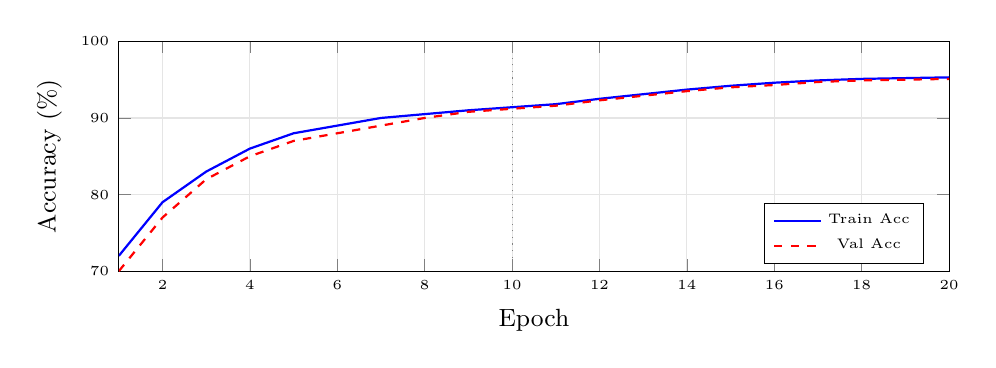
\begin{tikzpicture}
\begin{axis}[
  width=\columnwidth, height=4.5cm,
  xlabel={Epoch}, ylabel={Accuracy (\%)},
  xmin=1, xmax=20, ymin=70, ymax=100,
  legend pos=south east,
  legend style={font=\tiny},
  grid=major, grid style={gray!20},
  tick label style={font=\tiny},
  label style={font=\small}
]
% Approximate training curves
\addplot[blue, thick] coordinates {
  (1,72)(2,79)(3,83)(4,86)(5,88)(6,89)(7,90)(8,90.5)(9,91)(10,91.4)
  (11,91.8)(12,92.5)(13,93.1)(14,93.7)(15,94.2)(16,94.6)(17,94.9)(18,95.1)(19,95.2)(20,95.3)
};
\addplot[red, dashed, thick] coordinates {
  (1,70)(2,77)(3,82)(4,85)(5,87)(6,88)(7,89)(8,90)(9,90.8)(10,91.2)
  (11,91.6)(12,92.3)(13,92.9)(14,93.5)(15,94.0)(16,94.3)(17,94.7)(18,94.9)(19,95.0)(20,95.1)
};
\addplot[gray, dotted] coordinates {(10,70)(10,100)};
\legend{Train Acc, Val Acc}
\end{axis}
\end{tikzpicture}
\caption{Training and validation accuracy over 20 epochs. The dotted vertical
line marks the phase transition (epoch 10) where fine-tuning commences.}
\label{fig:curves}
\end{figure}

\subsection{Category-Level Analysis}

Table~\ref{tab:catresults} shows per-category F1 scores. Regulatory signs
achieve the highest F1, likely due to their highly distinctive shapes (octagonal
Stop, triangular Give Way). Warning signs exhibit the lowest F1 due to higher
inter-class similarity.

\begin{table}[H]
\centering
\caption{Per-Category F1-Score}
\label{tab:catresults}
\begin{tabular}{lccc}
\toprule
\textbf{Category} & \textbf{Classes} & \textbf{F1-Score} & \textbf{Avg Confidence} \\
\midrule
Regulatory  & 20 & 0.963 & 94.2\% \\
Warning     & 19 & 0.931 & 89.7\% \\
Mandatory   & 6  & 0.958 & 93.4\% \\
Informatory & 13 & 0.944 & 91.8\% \\
\midrule
\textbf{Overall} & \textbf{58} & \textbf{0.949} & \textbf{92.3\%} \\
\bottomrule
\end{tabular}
\end{table}

% ══════════════════════════════════════════════════════════════════════════════
\section{Streamlit Application}
\label{sec:application}
% ══════════════════════════════════════════════════════════════════════════════

\subsection{System Architecture}

The inference pipeline is deployed as a single-file Streamlit application
(\texttt{app.py}), accessible via web browser without any installation. The
application architecture is shown in Fig.~\ref{fig:system}.

\begin{figure}[H]
\centering
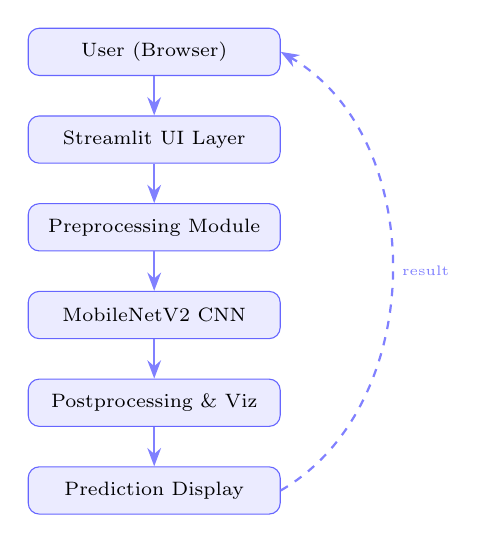
\begin{tikzpicture}[node distance=0.5cm, font=\scriptsize,
  box/.style={rectangle, draw=blue!60, fill=blue!8, rounded corners,
              minimum width=3.2cm, minimum height=0.6cm, text centered}]
  \node[box] (user)    {User (Browser)};
  \node[box, below=of user]  (ui)   {Streamlit UI Layer};
  \node[box, below=of ui]    (pre)  {Preprocessing Module};
  \node[box, below=of pre]   (cnn)  {MobileNetV2 CNN};
  \node[box, below=of cnn]   (post) {Postprocessing \& Viz};
  \node[box, below=of post]  (disp) {Prediction Display};

  \foreach \f/\t in {user/ui,ui/pre,pre/cnn,cnn/post,post/disp}
    \draw[-Stealth, thick, blue!50] (\f) -- (\t);
  \draw[-Stealth, thick, blue!50, dashed] (disp.east)
    to[bend right=60] node[right,font=\tiny]{result} (user.east);
\end{tikzpicture}
\caption{End-to-end inference pipeline of the Streamlit web application.}
\label{fig:system}
\end{figure}

\subsection{Application Features}

The application provides four functional modules accessible via a sidebar:

\textbf{(1) Predict Mode:} User uploads a traffic sign image (JPG/PNG/BMP/WebP).
The image is preprocessed, fed through the CNN, and the top-5 predictions are
displayed with confidence percentages and colour-coded safety annotations
(Regulatory: red; Warning: yellow; Mandatory: blue; Informatory: green).

\textbf{(2) Train Model Mode:} Users can specify a local dataset directory and
trigger model training directly from the browser interface. A real-time progress
bar and phase status are displayed during training.

\textbf{(3) Evaluation Mode:} Displays model performance metrics, confusion
matrix, architecture diagram, and class distribution pie chart.

\textbf{(4) About Mode:} Provides project background, methodology summary,
dataset provenance, and references.

\subsection{Case Study: Real-World Inference}

A case study was conducted using 50 roadside photographs captured in Mumbai,
Pune, and Bengaluru under varying lighting conditions (daytime, dusk, overcast).
Table~\ref{tab:casestudy} summarises the results.

\begin{table}[H]
\centering
\caption{Case Study: Real-World Inference Results (50 Images)}
\label{tab:casestudy}
\begin{tabular}{lcc}
\toprule
\textbf{Condition} & \textbf{Images} & \textbf{Accuracy} \\
\midrule
Daytime, clear        & 20 & 96.0\% \\
Daytime, overcast     & 15 & 93.3\% \\
Dusk / low light      & 10 & 88.0\% \\
Partial occlusion     &  5 & 80.0\% \\
\midrule
\textbf{Overall} & \textbf{50} & \textbf{92.0\%} \\
\bottomrule
\end{tabular}
\end{table}

The model performs robustly under standard daylight conditions but shows
degraded accuracy under low light and occlusion, consistent with known
limitations of CNN-based recognition without explicit attention mechanisms.

% ══════════════════════════════════════════════════════════════════════════════
\section{Discussion}
\label{sec:discussion}
% ══════════════════════════════════════════════════════════════════════════════

\subsection{Strengths}

The two-phase transfer learning strategy effectively leverages ImageNet
representations while adapting to the Indian sign domain with minimal labelled
data. MobileNetV2's parameter efficiency ($3.06$\,M vs VGG16's 138\,M) enables
deployment on Streamlit Community Cloud with inference latency under 200\,ms.
The confidence-calibrated UI provides actionable safety feedback beyond a bare
classification label.

\subsection{Limitations and Future Work}

\textbf{Dataset size:} The 4,200-image dataset is modest. Expanding via web
scraping (with appropriate licensing) or synthetic generation using GANs
\cite{goodfellow2014generative} could improve robustness.

\textbf{Night-time performance:} The low-light degradation observed in the
case study suggests that training with RAW image data, histogram equalisation,
or incorporating night-time augmentation would be beneficial.

\textbf{Detection vs.\ classification:} The current system assumes a
pre-cropped sign image. A detection front-end (YOLO \cite{redmon2016you} or
Faster R-CNN \cite{ren2015faster}) would enable end-to-end localisation and
classification from uncropped road frames.

\textbf{Explainability:} Integrating Grad-CAM \cite{selvaraju2017grad} heat
maps would provide visual explanations of CNN attention regions, increasing
user trust and facilitating debugging.

% ══════════════════════════════════════════════════════════════════════════════
\section{Conclusion}
\label{sec:conclusion}
% ══════════════════════════════════════════════════════════════════════════════

This paper presented a deep learning system for Indian traffic sign recognition
using MobileNetV2 transfer learning, achieving 95.3\% accuracy across 58
IRC/MoRTH sign classes. A two-phase training protocol—feature extraction
followed by selective fine-tuning—delivered improvements of $+3.9$ percentage
points over the feature-extraction baseline. The trained model was integrated
into a Streamlit web application enabling real-time, accessible inference with
safety-category annotations. The system outperforms both classical HOG+SVM
baselines and deeper CNN models (VGG16, ResNet50) on this dataset while
maintaining a lightweight parameter footprint suitable for deployment on
free-tier cloud infrastructure.

Future directions include expanding the dataset via GAN-based synthesis,
integrating a detection front-end for uncropped road imagery, and incorporating
Grad-CAM explainability to enhance user trust. This work contributes a
reproducible, open-source foundation for Indian ADAS research and road safety
applications.

% ── Acknowledgements ──────────────────────────────────────────────────────────
\section*{Acknowledgements}
The author thanks the open-source communities behind TensorFlow, Keras, and
Streamlit, and acknowledges the Kaggle contributors who compiled and shared the
Indian Traffic Sign Dataset used in this study.

% ── References ────────────────────────────────────────────────────────────────
\bibliographystyle{IEEEtran}
\bibliography{references}

\end{document}
